\section{Architectural Design}
\subsection{Block diagram}
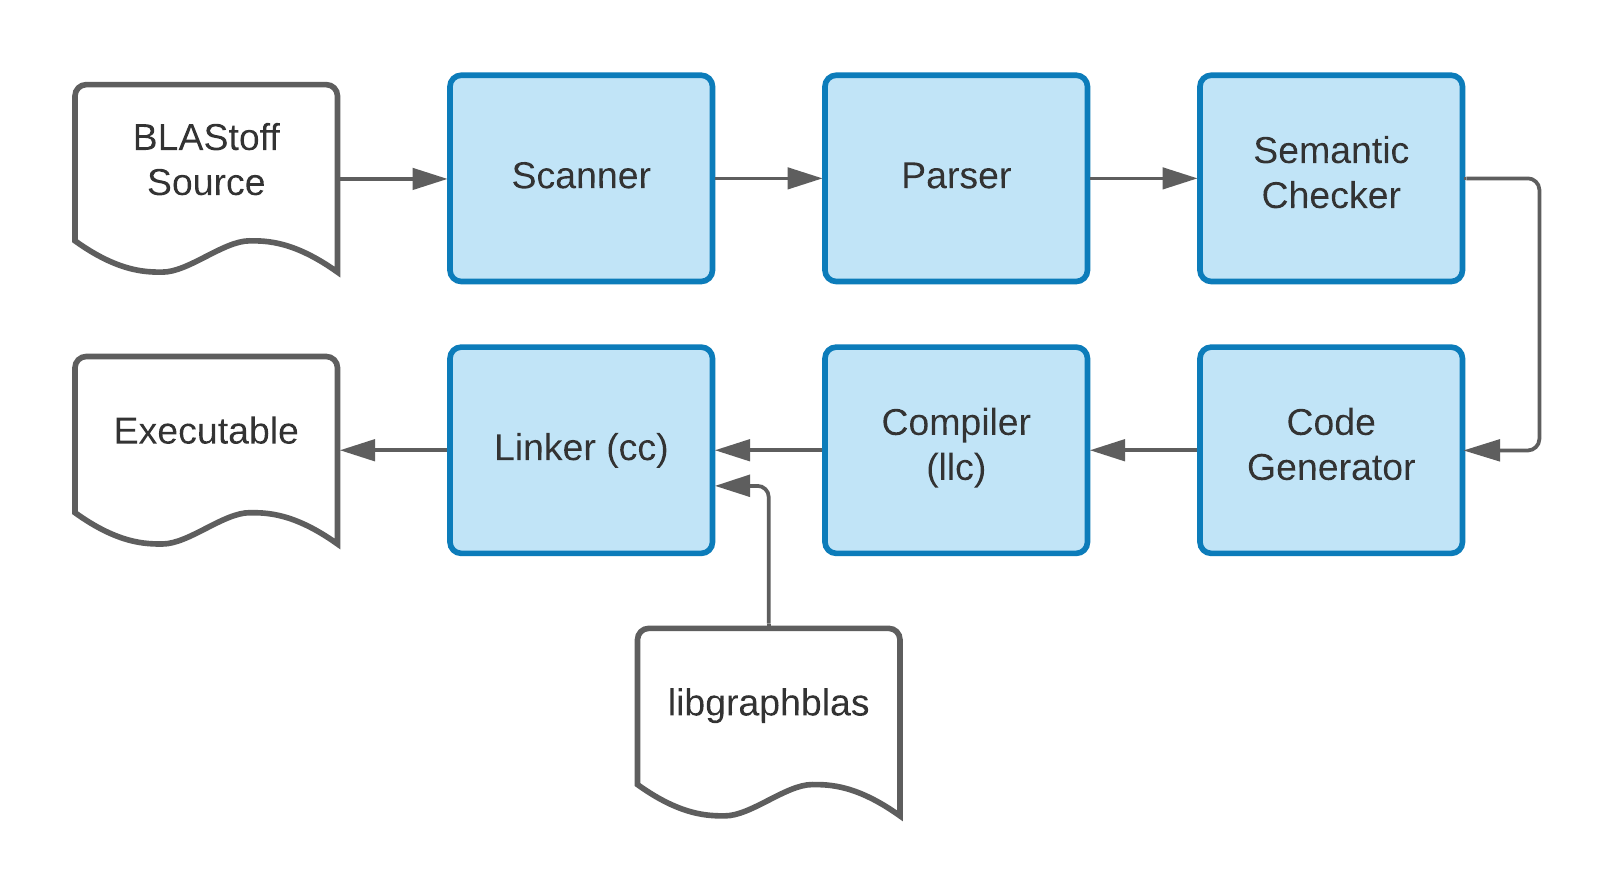
\includegraphics[width=\textwidth]{figures/block-diagram.png}
\subsection{Scanner}
The scanner takes raw BLAStoff source and breaks it into tokens. In doing
so, it removes whitespace (which is no longer needed once the tokens have
been found) and comments. It is possible for syntactically incorrect code to
be successfully scanned, as long as the tokens themselves are valid BLASToff
tokens.

Built by Katon, Michael, Jake, Jason

\subsection{Parser}
The parser takes the tokens generated by the scanner and outputs an abstract
syntax tree (AST) according to the BLAStoff grammar. If the code is
syntactically incorrect, the parser will throw an error. However, semantic
errors may not be caught at this stage.

Built by Katon, Jake, Jason, Michael

\subsection{Semantic Checker}
Our semantic checker takes the AST from the parser and ensures that it is
semantically correct. For example, we use a symbol table to throw an error
at this stage if a symbol is used before it is declared. Because our
language technically has only one type (matrix), we decided to forgo the
SAST, i.e. we do not annotate types in this stage. Thus, assuming that the
it passes semantic checking, the AST is not modified in this step.

Built by Katon, Jake, Jason, Michael

\subsection{Code Generator}
The code generator takes the AST and generates LLVM IR code. Note that many
of our matrix operations and semiring manipulations turned into calls to our
C backend.

The code generator (written in OCaml) was built by Katon, Michael, Jake, and
Jason. The C backend was built by Michael and Jake.

\subsection{Compiler and Linker}
The compiler uses the LLVM IR code to generate machine code that is then
linked with the GraphBLAS library to create the final executable.
